Der skill-basierte Ansatz beinhaltet eine Vielzahl unterschiedlicher Aspekte. Für die Thesis ist es daher entscheidend, die Prioritäten klar zu setzen. Zur strukturierten Bearbeitung werden verschiedene Arbeitspakete festgelegt, die die zentralen Anforderungen des Projekts abdecken. Im Anschluss werden die Abhängigkeiten dieser Arbeitspakete bestimmt und in einem Gate-Plan visualisiert. Dieser gliedert die Bearbeitung in Phasen und zeigt die Reihenfolge auf, in der die Arbeitspakete abgearbeitet werden sollen.


\section{Arbeitspakete} \label{Arbeitspakete}

	Grundsätzlich teilt sich das Gesamtsystem in die Hardware und Software ein. Diese lassen sich anschliessend in verschiedene Arbeitspakete einteilen. 

	\begin{figure}[h!]
		\centering
		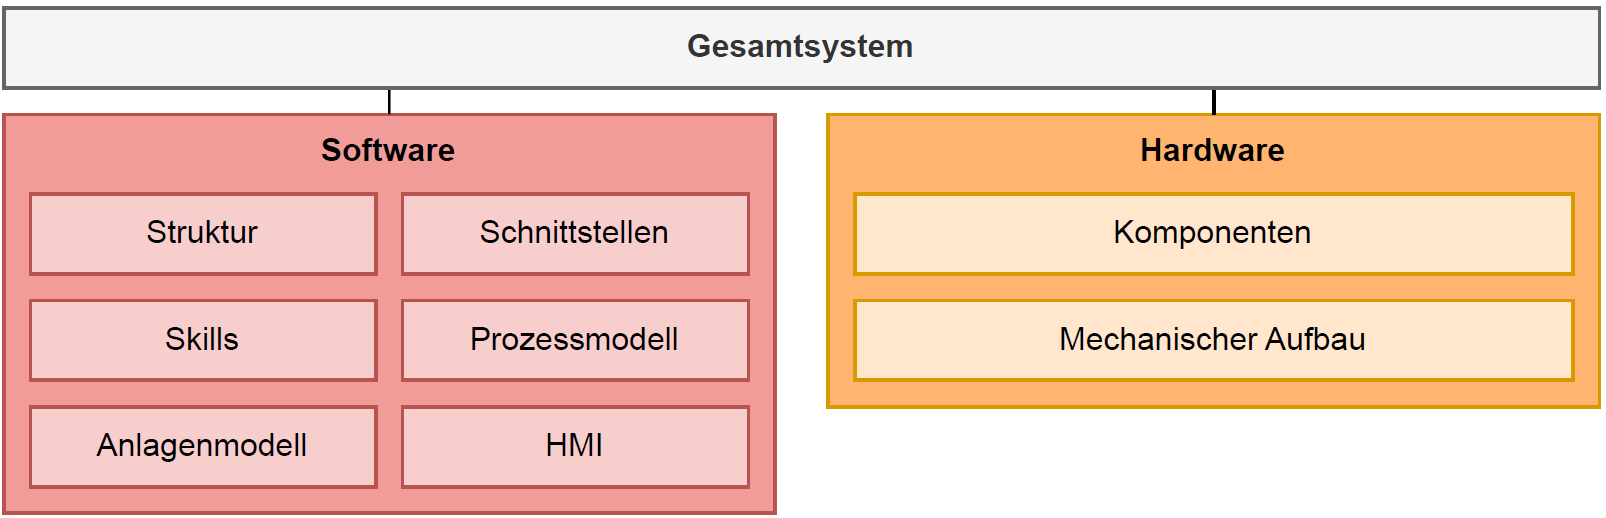
\includegraphics[width=0.5\textwidth]{03_Vorgehen_fuer_die_Thesis/Arbeitspakete}
		\captionsetup{justification=centering}
		\caption{Definierte Arbeitspakete}
		\label{fig:Arbeitspakete}
	\end{figure}
	
	\newpage

